% !TeX program = xelatex
\documentclass[a4paper, 12pt]{article}

\usepackage[brazil]{babel}
\let\latinencoding\relax
\usepackage[T1]{fontenc}

\usepackage[no-math]{fontspec}
\usepackage{newpxtext, newpxmath}
\usepackage[a4paper, margin=2cm]{geometry}
\usepackage{pdflscape}
\usepackage{graphicx}
\usepackage{float}
\usepackage{rotating}
\usepackage{pdflscape}
\usepackage[colorlinks,urlcolor=blue,linkcolor=black]{hyperref}

\input{definition.tex}

\title{\titulo}
\author{\nomeAutorUm e \nomeAutorDois}
\date{\today}

\newcommand{\printtitle}{
  \begin{center}
    {\Large \scshape \titulo}\\[1em]
    {\nomeAutorUm, \raAutorUm}\\   
    {\nomeAutorDois, \raAutorDois}\\   
    {\bfseries Turma: \turma{} -- \periodo}\\[0.5em]
    Professor: Dr\@. \nomeProfessorUm, \centroProfessor\\
    Professor: Dr\@. \nomeProfessorDois, \centroProfessor\\    
    {\itshape \campusFaculdade}
  \end{center}
}

\begin{document}
  \printtitle

  \section{Introdução}

  O projeto consiste em realizar uma implementação visual 
  do jogo Tetris em Java, através do pacote \texttt{javax.swing}.
  O objetivo principal é modelar as classes de um jeito que
  todo o comportamento do jogo seja realizado por classes
  respectivas e as classes do visual apenas tenham uma
  ligação simples, acessando apenas alguns atributos e
  controlando o jogo com os métodos providenciados, dividindo
  assim as responsabilidades e aumentando a coesão.

  \section{Descrição das classes}

  O projeto divide as responsabilidades do gerenciamento
  do jogo e do visual, através das classes nos pacotes
  \texttt{tetris} e \texttt{gui}, respectivamente. As
  principais classes do projeto são:

  \begin{itemize}
    \item Pacote \texttt{tetris}:

    \begin{itemize}
      \item
      \texttt{Bloco}: representa cada bloco, com suas posições
      e cores, de uma \texttt{Peca}.

      \item
      \texttt{Peca}: classe base para as peças disponíveis
      por padrão, assim como as criadas pela reação em cadeia.

      \item
      \texttt{FloodFill}: classe responsável pela execução
      do algoritmo \emph{Flood Fill} no tabuleiro para a 
      reação em cadeia.

      \item
      \texttt{Tabuleiro}: classe responsável pelo jogo, representa
      o tabuleiro com uma matriz de blocos e permite a interação
      do mundo externo com o jogo, através dos métodos de controle.

      \item
      \texttt{AuxiliarTabuleiro}: métodos auxiliares para
      o funcionamento do \texttt{Tabuleiro}.
    \end{itemize}

    \item Pacote \texttt{gui}:

    \begin{itemize}
      \item
      \texttt{PanelBase}: implementação personalizada do
      \texttt{JPanel}, do Java, com o \emph{design} base
      para todas as telas da interface visual.

      \item
      \texttt{PanelInicio}: tela inicial do jogo, que
      permite escolher a dificuldade desejada.

      \item
      \texttt{PanelJogo}: tela do jogo, que mostra
      o tabuleiro através do \texttt{PanelTabuleiro}
      e as informações básicas, como o placar.

      \item
      \texttt{PanelTabuleiro}: painel responsável apenas
      pelo desenho do tabuleiro do jogo.

      \item
      \texttt{PanelGameOver}: tela de \emph{game over}
      do jogo, que mostra o placar final e permite
      a escolha entre jogar novamente na mesma dificuldade
      ou voltar para o início.

      \item
      \texttt{JanelaPrincipal}: janela que mostra as
      telas de início, jogo ou \emph{game over}.
    \end{itemize}
  \end{itemize}

  \begin{landscape}
  \begin{figure}
    \centering
    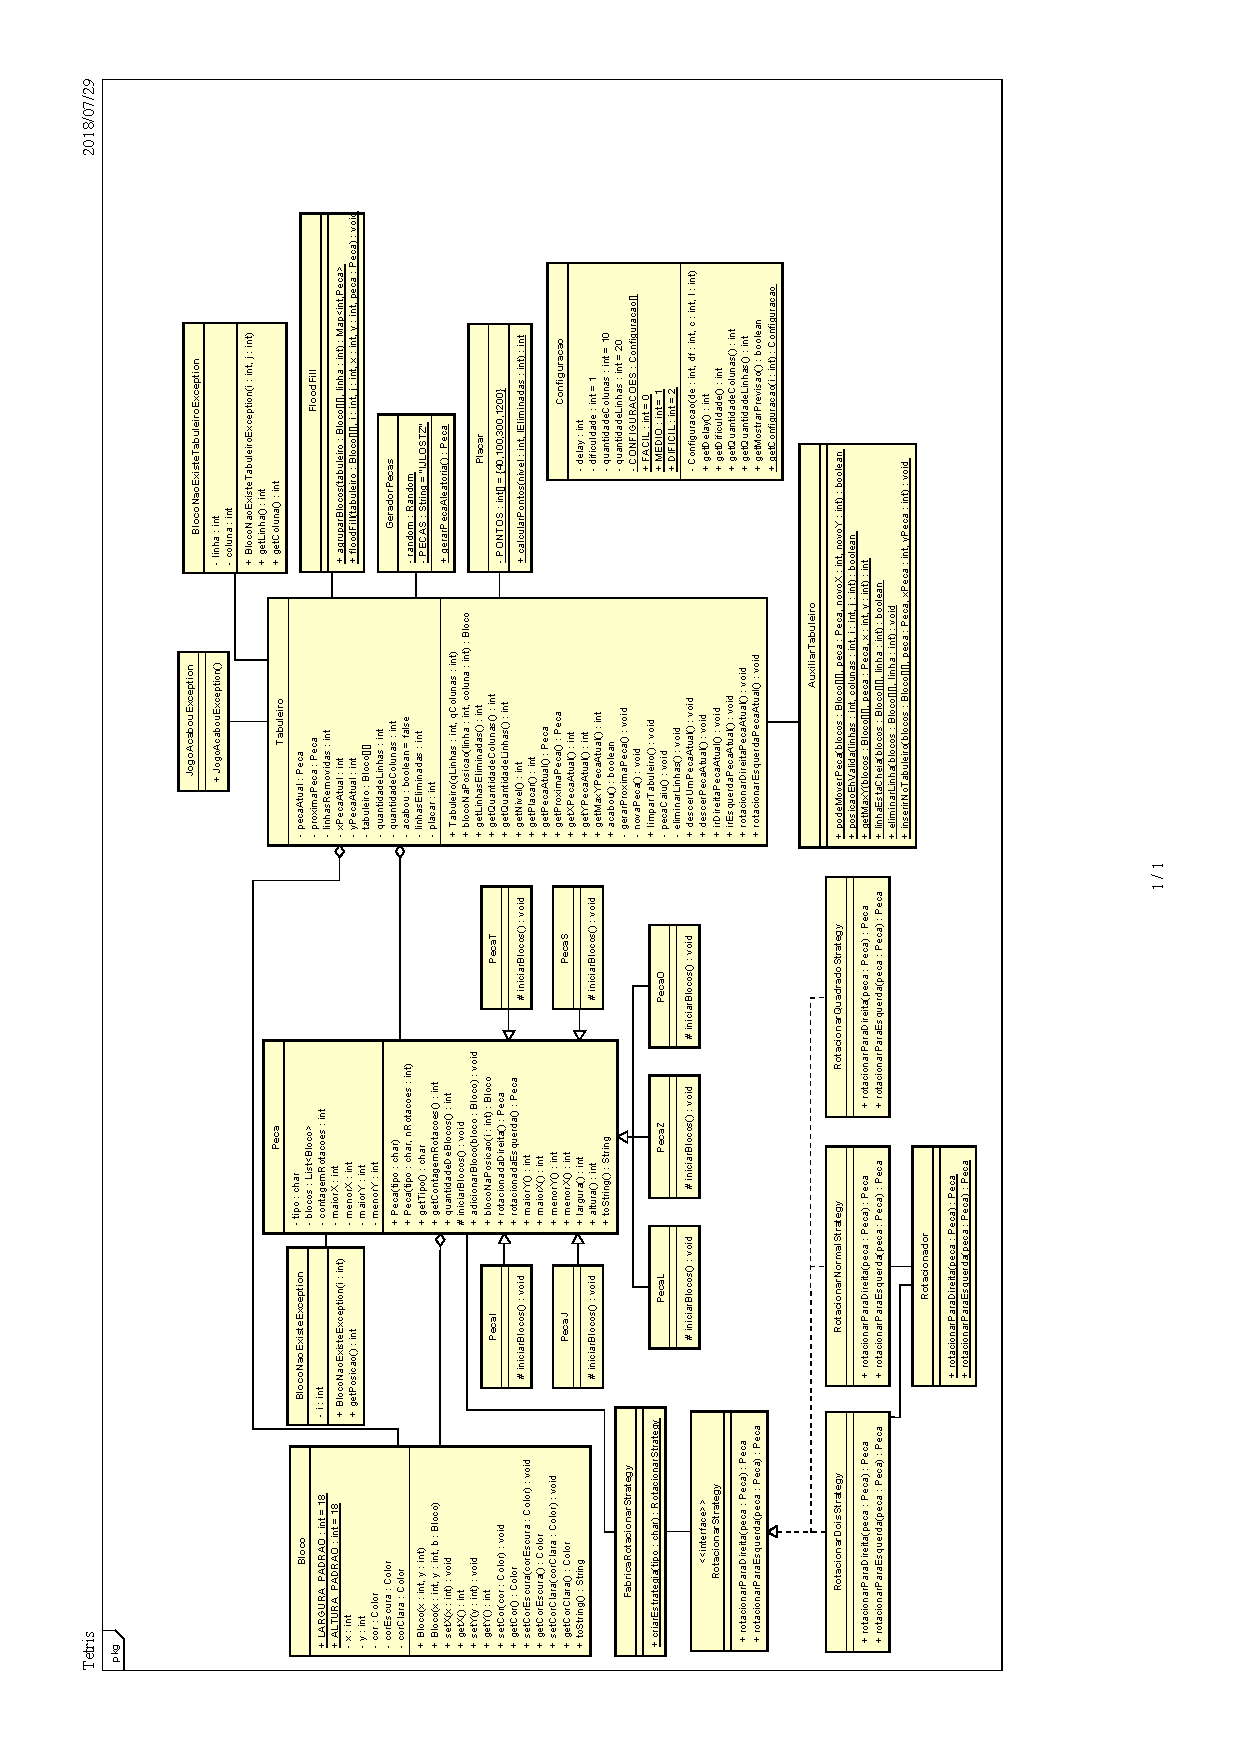
\includegraphics[angle=-90,trim=2.2cm 1.5cm 4.3cm 3cm,clip]{diagram/package-tetris.pdf}
    \caption{Diagrama UML do pacote \texttt{tetris}.}
  \end{figure}
  \end{landscape}

  \begin{landscape}
  \begin{figure}
    \centering
    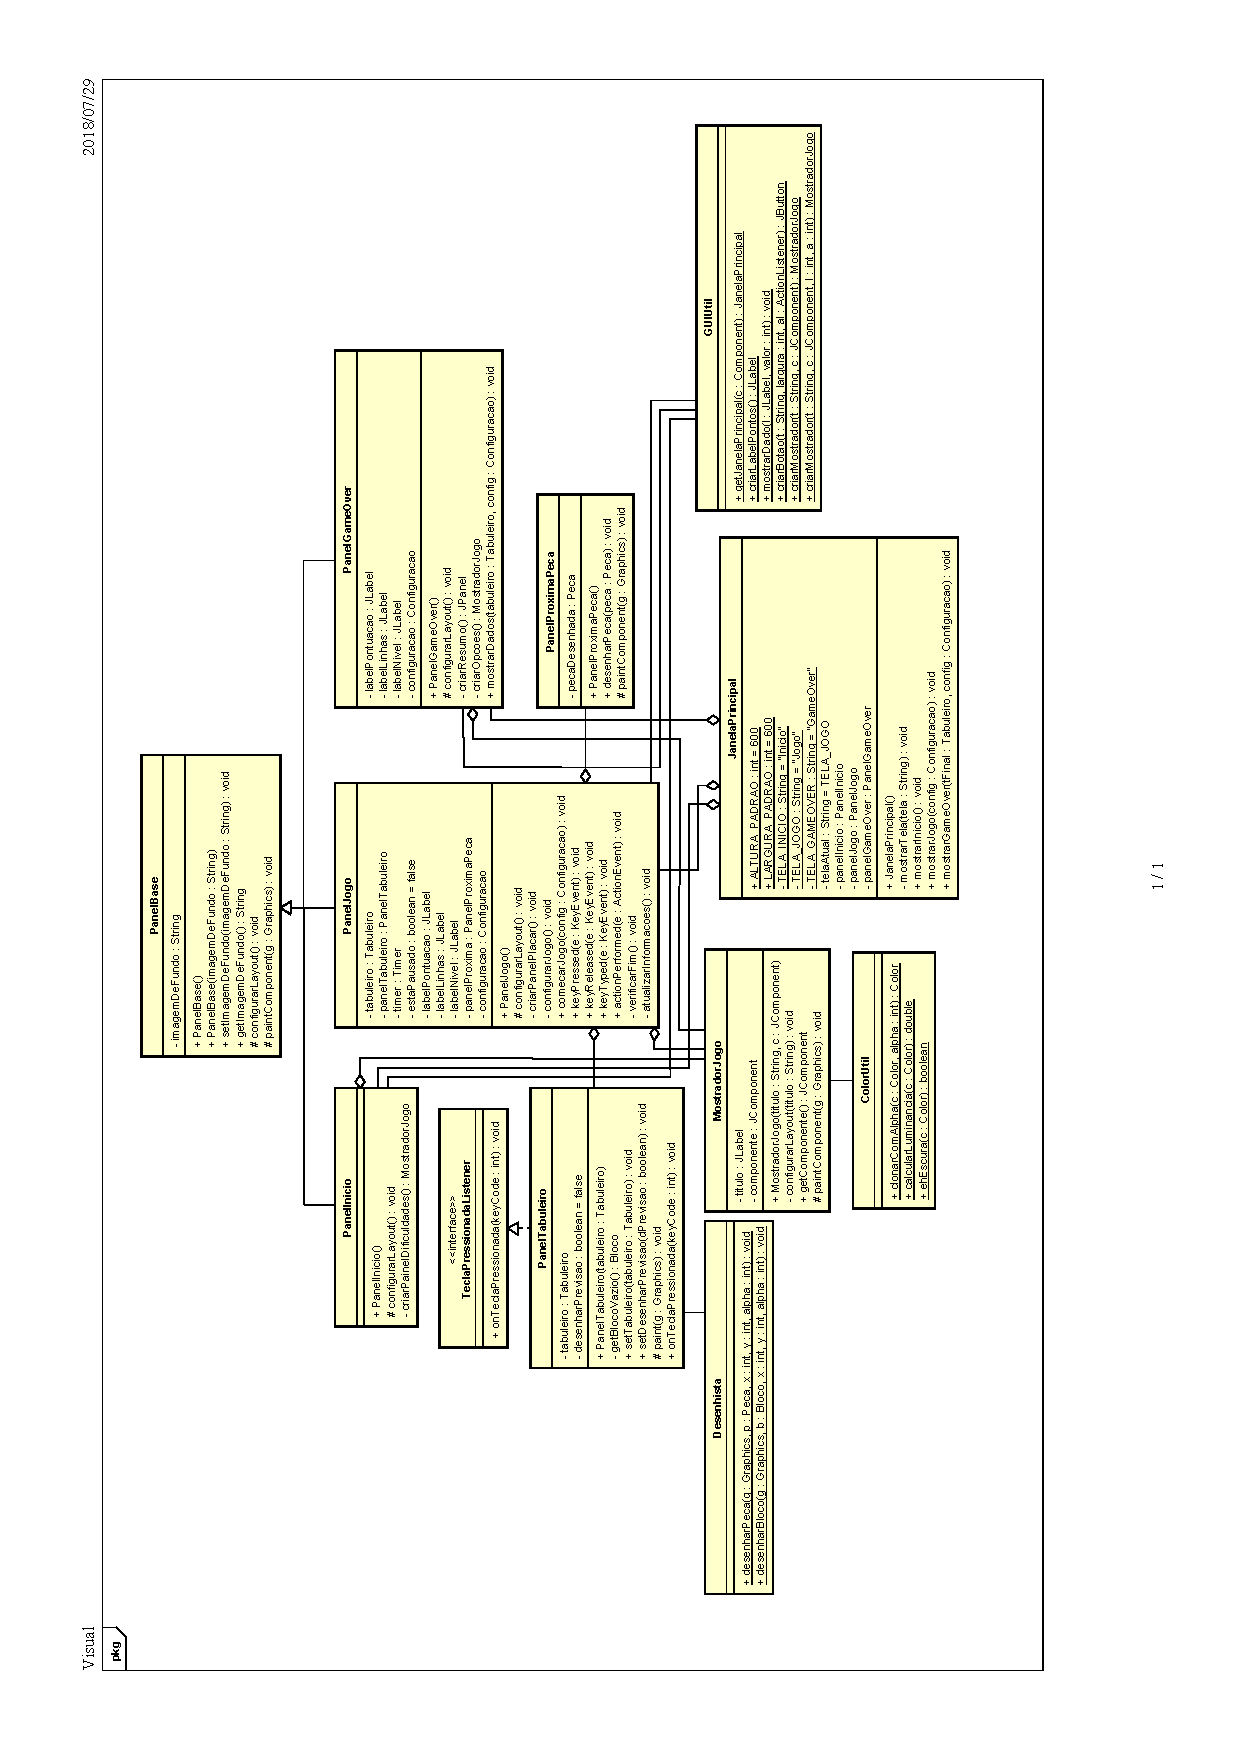
\includegraphics[angle=-90,trim=2.3cm 2cm 4cm 2cm,clip]{diagram/package-gui.pdf}
    \caption{Diagrama UML do pacote \texttt{gui}.}
  \end{figure}
  \end{landscape}

  \section{Conceitos de orientação a objetos aplicados}

  As classes responsáveis por cada peça do jogo usam o conceito de herança,
  já que todas herdam as características da classe base \texttt{Peca}.
  Cada classe que herda sobrescreve o método \texttt{iniciarBlocos()},
  que permite que os blocos customizados sejam criados para cada tipo
  de peça. O mesmo conceito  é utilizado nas classes responsáveis pelos
  três painéis principais no visual (\texttt{PanelInicio}, \texttt{PanelJogo} 
  e \texttt{PanelGameOver}), onde as mesmas herdam de \texttt{PanelBase},
  sobrescrevendo o método \texttt{configurarLayout()}.

  O conceito de agregação é utilizado nas relações \texttt{Bloco}--\texttt{Peca},
  \texttt{Bloco}--\texttt{Tabuleiro} e \texttt{Peca}--\texttt{Tabuleiro},
  já que o ``todo'' possui as partes, mas caso o ``todo'' for eliminado,
  ainda é possível utilizá-las. Já no pacote \texttt{gui}, a agregação
  é utilizada em: \texttt{PanelInicio}, \texttt{PanelJogo} e \texttt{PanelGameOver}
  com \texttt{JanelaPrincipal}; \texttt{MostradorJogo} com \texttt{PanelInicio}, 
  \texttt{PanelJogo} e \texttt{PanelGameOver}; \texttt{PanelProximaPeca}
  com \texttt{PanelJogo}; e \texttt{PanelTabuleiro} com \texttt{PanelJogo}.

  A classe \texttt{Tabuleiro} depende de muitos métodos específicos,
  portanto, para aumentar a coesão, optou-se por criar classes específicas
  apenas com esses intuitos, tais como \texttt{FloodFill}, \texttt{GeradorPecas}
  e \texttt{Placar}. Do mesmo modo, os três pricipais painéis do visual
  compartilham métodos em comum, utilizando então uma classe específica
  auxiliar como apoio, a \texttt{GUIUtil}.

  O \texttt{PanelTabuleiro} implementa a interface \texttt{TeclaPressionadaListener},
  assim, quando os eventos de teclas pressionadas são capturados em \texttt{PanelJogo},
  através do método implementado \texttt{keyPressed()} de \texttt{KeyListener},
  os mesmos são enviados para o \texttt{PanelTabuleiro} através do método
  \texttt{onTeclaPressionada()}, para então realizar o tratamento das teclas.

  Algumas peças, como a Z, S, I e O possuem comportamentos diferentes em
  relação as suas rotações: Z, S e I possuem somente dois ``estados'',
  que ficam alternando entre si; e O possui apenas um ``estado'', ela
  não possui rotações. As demais peças, T, J e L, possuem um comportamento
  normal de rotações, ou seja, possuem os quatro ``estados'', como pode-se
  observar na Figura \ref{fig:rotacoes}.
  
  \begin{figure}[ht]
    \centering
    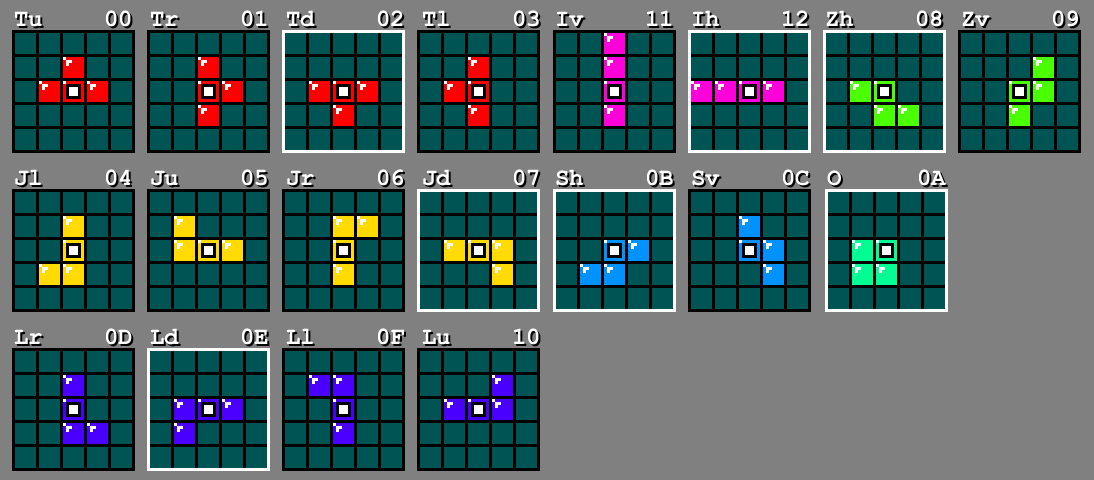
\includegraphics[width=0.9\textwidth]{0.png}
    \caption{Tabela de rotações das peças. Fonte: \url{http://bit.ly/2NQAuum}.}
    \label{fig:rotacoes}
  \end{figure}

  Para contornar esse problema, optou-se por utilizar o padrão de projeto
  \emph{Strategy}. A interface \texttt{RotacionarStrategy} possui dois
  métodos: um para rotacionar uma peça dada para a esquerda e um para a direita.
  Assim, pôde-se definir três implementações desta estratégia:
  a \texttt{RotacionarDoisStrategy}, que fica alternando entre as rotações
  com base no atributo \texttt{contagemRotacoes} da \texttt{Peca}; a
  \texttt{RotacionarQuadradoStrategy}, que apenas retorna a mesma
  peça dada como parâmetro em seus métodos; e a \texttt{RotacionarNormalStrategy},
  que rotaciona a peça, tanto para a direita, quanto para a esquerda,
  em seus quatro ``estados'' possíveis. Como a \texttt{RotacionarNormalStrategy}
  e a \texttt{RotacionarDoisStrategy} utilizam como base o mesmo algoritmo
  de rotacionamento para a esquerda e direita, abstraiu-se este algoritmo
  para uma classe responsável somente por isto, a classe \texttt{Rotacionador}.
  Então, para efetuar as rotações, na classe base \texttt{Peca}, nos métodos
  \texttt{rotacionadaDireita()} e \texttt{rotacionadaEsquerda()}, chama-se
  o método respectivo da estratégia do tipo de peça. Para isso, existe
  a classe \texttt{FabricaRotacionarStrategy} que cria uma estratégia
  com base no tipo especificado e retorna-a. Então, de certo modo, pode-se
  dizer que esta classe é uma versão mais simples do padrão de projeto \emph{Factory},
  já que ela é responsável em criar a estratégia correta com base no tipo.

  Há também o lançamento de exceções do tipo \emph{unchecked} quando tenta-se
  acessar algum bloco em uma posição inválida no \texttt{Tabuleiro} ou
  na \texttt{Peca}. Da mesma forma, quando tenta-se realizar algum controle
  no \texttt{Tabuleiro} quando o jogo já terminou, é lançada a exceção
  \texttt{JogoAcabouException}.

  É interessante notar que há uma separação de responsabilidades entre
  os pacotes \texttt{tetris} e \texttt{gui}. A interface visual apenas
  utiliza os métodos do \texttt{Tabuleiro} para se comunicar com ele
  e controlar o jogo baseando-se nas teclas. No entanto, caso fosse
  necessário construir uma interface visual em outro estilo, como
  uma no console ou utilizando JavaFX, poderia-se facilmente
  criar somente a interface visual e utilizar os mesmos métodos
  de comunicação que a atual, feita em Swing, utiliza.

  \section{Participação de cada integrante do grupo}

  As contribuições foram divididas em:

  \begin{description}
    \item[Alessandro] estudo do funcionamento do \emph{Tetris};
    modelagem básica inicial das classes do jogo,
    bem como suas implementações elementares; desenvolvimento da 
    interface visual; revisão do diagrama de classes;
    confecção do relatório.

    \item[Victor] aperfeiçoamento da modelagem das classes;
    implementação da reação em cadeia através do algoritmo
    \emph{Flood Fill}; implementação e aperfeiçoamento
    das demais classes; geração do diagrama de classes;
    revisão do relatório;
  \end{description}
\end{document}